\section{REGISTER}
    Στη σελίδα \texttt{signup.html} ορίζεται η φόρμα εγγραφής των χρηστών-πολιτών:

    \begin{figure}[H] \noindent \centering
        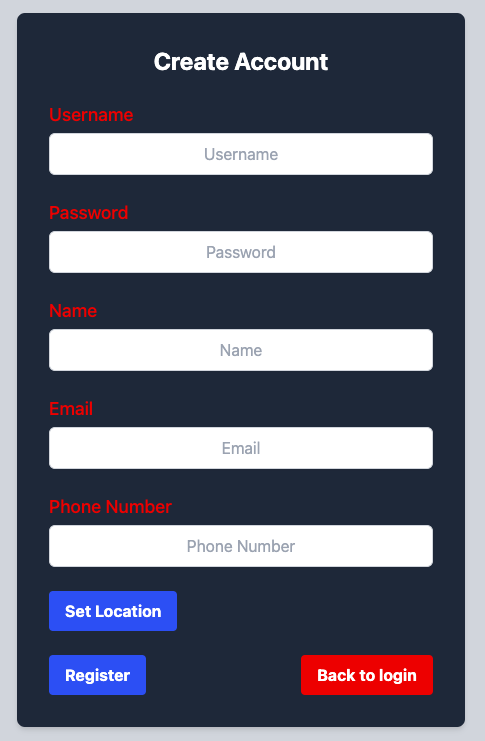
\includegraphics[width=0.3\textwidth]{img/register}
        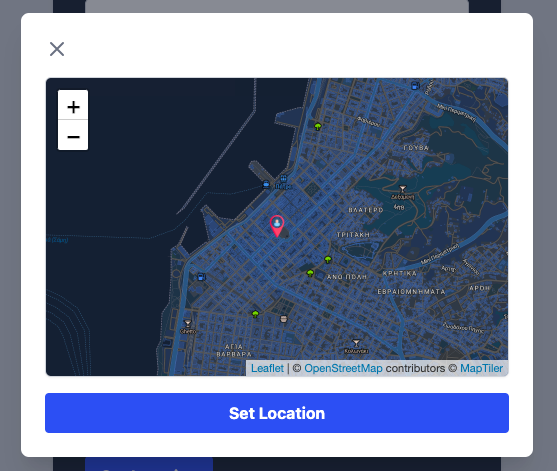
\includegraphics[width=0.3\textwidth]{img/register-location}
        \caption{Σελίδα Signup και modal προσδιορισμού τοποθεσίας}
    \end{figure}

    \subsection{\texttt{signup.js}}
        Η συνάρτηση \texttt{signup()} δέχεται τα ορίσματα των input fields, ελέγχει αν έχουν πληροφορία (αν δεν έχουν, στέλνεται alert),
            και αν έχουν, στέλνει ένα AJAX request στο \texttt{register\_user.php}.

        Οι συναρτήσεις \texttt{openModal()} και \texttt{closeModal()}, εμφανίζουν και αποκρύπτουν το modal προσδιορισμού τοποθεσίας,
            το οποίο εμφανίζεται πατώντας στο κουμπί \textbf{Set Location}.
        Αυτό επιτυγχάνεται με την κατάλληλη αφαίρεση και προσθήκη κλάσεων του Tailwind CSS.

        Στην εμφάνιση του \textbf{Set Location}, αρχικοποιείται ο χάρτης μέσω της \texttt{initializeMap()}.
        Ορίζεται η σταθερά \texttt{map} μέσω της Leaflet, με κεντραρισμένο view στο κέντρο της Πάτρας.
        Ορίζεται ο χάρτης που θα χρησιμοποιήσουμε ως συγκεκριμένο \texttt{tileLayer} (ο οποίος χάρτης εξάγεται μέσω API από το maptiler.com),
            και προστίθεται ένα marker (\texttt{userIcon} που αντιστοιχεί στην εικόνα \texttt{user.png}), το οποίο αρχικοποιείται με αρχική θέση στο κέντρο της Πάτρας (ίδιο location με την αρχικοποίηση του view).
        Ελέγχεται το event του \texttt{click}, και σε εκείνη την περίπτωση αποθηκεύονται οι αλλαγμένες συντεταγμένες ως value στο \texttt{input} με \mbox{\texttt{id = location}}.

    \subsection{\texttt{register\_user.php}}
        Αφού ανακτηθούν οι πληροφορίες, γίνονται insert στη βάση δεδομένων και γίνεται echo μήνυμα επιτυχίας.
        Στην περίπτωση της μεταβλητής της τοποθεσίας, είναι αναγκαία η διάσπασή της σε ξεχωριστές μεταβλητές για το \texttt{latitude} και \texttt{longitude}.

